\documentclass[12pt,letterpaper]{article}
\usepackage[latin1]{inputenc}
\usepackage{amsmath}
\usepackage{amsfonts}
\usepackage{amssymb}
\usepackage{amsthm}
\usepackage{enumerate}
\usepackage[margin=0.8in]{geometry}
\usepackage{graphicx}

\newtheorem{theorem}{Theorem}[section]
\newtheorem{rem}[theorem]{Remark}
\newenvironment{remark}{\begin{rem}\rm}{\end{rem}}
\newtheorem{claim}[theorem]{Claim}
\newtheorem{lemma}[theorem]{Lemma}
\newtheorem{proposition}[theorem]{Proposition}
\newtheorem{corollary}[theorem]{Corollary}
\newtheorem{eg}[theorem]{Example}
\newenvironment{example}{\begin{eg}\rm}{\end{eg}}
\newtheorem{definition}[theorem]{Definition}

\newcommand{\C}{\mathbb{C}}
\newcommand{\R}{\mathbb{R}}
\newcommand{\x}{\mathbf{x}}
\renewcommand{\r}{\mathbf{r}}
\newcommand{\abs}[1]{\lvert#1\rvert}
\DeclareMathOperator{\Real}{Re}
\DeclareMathOperator{\Img}{Im}
\author{Sean Fitzpatrick}
\title{Oriented curves and some basic topology}

\begin{document}
\maketitle
\begin{abstract}
We give a summary of definitions and properties related to oriented curves in $\R^n$, and then discuss the notion of connected and simply connected sets.
\end{abstract}
\section{Oriented curves in $\R^n$}
Let $C$ be a bounded curve in $\R^n$, so that the boundary of $C$ is either empty, or a two-point set $\partial C=\{\x_0,\x_1\}$ consisting of the endpoints of $C$. (If the boundary of $C$ is empty, then $C$ is known as a {\em closed curve}; we will discuss closed curves below. Assume that $C$ has non-empty boundary. An {\em orientation} of $C$ is a choice of initial point from $\partial C$; thus, it is clear that a curve can have two possible orientations. A curve $C$ together with a choice of orientation is known as an {\em oriented curve}. The oriented curve with the opposite orientation is denoted by $-C$.
\begin{center}
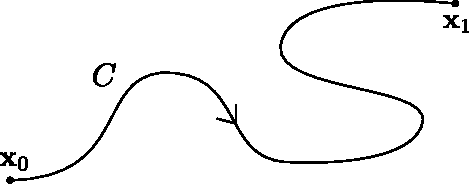
\includegraphics[width=2.6in]{oriented.pdf}
\end{center}
Suppose $C$ is an oriented curve with initial point $\x_0$. A {\em parameterization} of $C$ is a map $\mathbf{r}:[a,b]\to \R^n$ whose image is $C$, such that $\r(a)=\x_0$ and $\r(b)=x_1$. If $\r(t)$ is of class $C^1$ (that is, $\r\,'(t)$ exists and is continuous), and $\r\,'(t)\neq \mathbf{0}$ for all $t\in (a,b)$, then we say that the oriented curve $C$ is {\em smooth}.
\begin{remark}
The requirement that $\r\,'(t)\neq \mathbf{0}$ ensures that the curve $C$ cannot have any corners or cusps. If we allow $\r\,'(t)$ to vanish, then it is possible for the curve $C$ to have a corner while $\r$ remains $C^1$, by having $\r\,'$ approach the zero vector from either side of the corner. Note that this also means that a smooth curve cannot ``double back'' on itself: if $\r\,'(t_1)=\x_1$ for some $t_1\neq b$, then we would have to have $\r\,'(t_1)=\mathbf{0}$. (A ``particle'' on the curve would have to stop in order to turn around and go back the way it came.)
\end{remark}
By the above remark, a smooth oriented curve $C$ cannot have corners or reverse direction. However, this is allowed for a {\em piecewise-smooth} oriented curve. Note that although a smooth curve cannot reverse direction, it can intersect itself at some finite number of points. When this happens, we say that the curve is {\em non-simple}.
\begin{definition}
A continuous oriented curve $\r:[a,b]\to\R^n$ is called {\bf piecewise-smooth} if there exist points $a_0=a<a_1<\ldots <a_n=b$ such that $\r$ is differentiable on $(a_i,a_{i+1})$ for each $i$, and $\r'$ is continuous on $[a_i,a_{i+1}]$ (which means that $\lim\limits_{t\to a_i^+}\r'(t)$ and $\lim\limits_{t\to a_{i+1}^-}\r'(t)$ exist).  We say that $\r$ is {\bf closed} if $\r(a)=\r(b)$, and {\bf simple} if $\r(t_1)\neq \r(t_2)$ for any $a<t_1,t_2<b$.
\end{definition}
\begin{center}
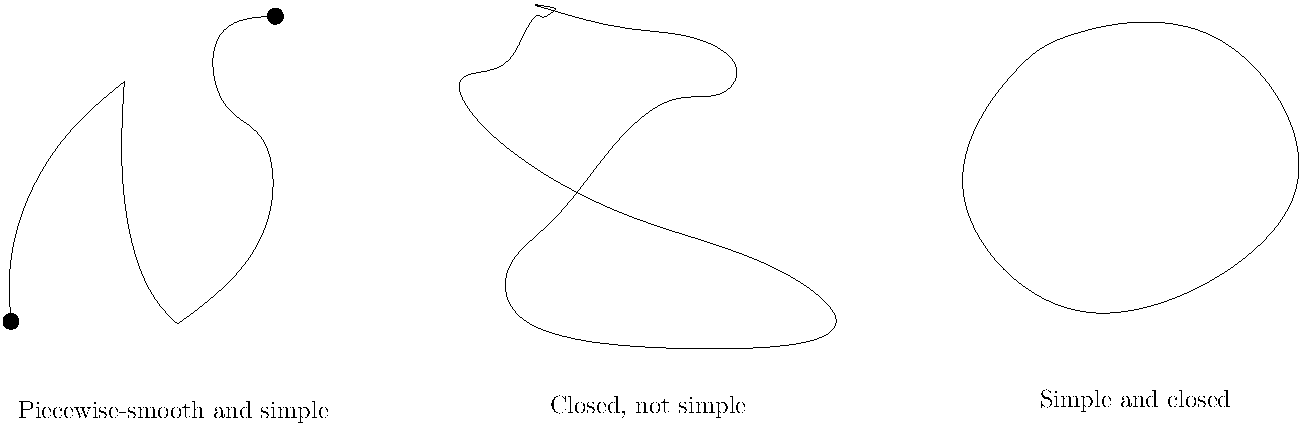
\includegraphics[width=5.5in]{curves_eg.pdf}
\end{center}
Note that $\r$ is a piecewise function, made up of $C^1$ functions $\r_i:[a_{i-1},a_i]$. The image of each $\r_i$ is a smooth oriented curve $C_i$, and the curves $C_i$ are such that the final point of $C_i$ is equal to the initial point of $C_{i+1}$. To indicate that $C$ is formed by joining together the smooth curves $C_1, \ldots, C_n$, we write $C=C_1+\cdots +C_n$.

If two oriented smooth curves $C_1$ and $C_2$ have the same final point, then the oriented curve $-C_2$ has the same initial point as the final point of $C_1$, and we can form the piecewise-smooth oriented curve $C_1+(-C_2)$, which we denote simply by $C_1-C_2$. We can similarly form the piecewise-smooth curve $C_2-C_1$, and the same argument holds if $C_1$ and $C_2$ have the same initial point.
\begin{remark}
Given a $C^0$ function $f$ or vector field $\mathbf{F}$ defined along a piecewise smooth curve $C$ as above, we define
\begin{align*}
\int_C f ds &= \int_{C_1+\cdots +C_n} f ds = \int_{C_1} f ds + \cdots +\int_{C_n} f ds, \text{ and }\\
\int_C \mathbf{F}\cdot d\r &= \int_{C_1+\cdots +C_n} \mathbf{F}\cdot d\r = \int_{C_1} \mathbf{F}\cdot d\r+\cdots +\int_{C_n}\mathbf{F}\cdot d\r.
\end{align*}
Moreover, we have
\[
\int_{-C}\mathbf{F}\cdot d\r = -\int_{C}\mathbf{F}\cdot d\r, \quad \int_{C_1-C_2}\mathbf{F}\cdot d\r = \int_{C_1}\mathbf{F}\cdot d\r-\int_{C_2}\mathbf{F}\cdot d\r.
\]
However, note that $\displaystyle \int_{-C} fds = \int_{C}fds$, so that line integrals of scalar functions do not depend on the orientation of the curve $C$.
\end{remark}
As noted above, a smooth closed curve $C$ is parameterized by a $C^1$ function $\r$ such that $\r(a)=\r(b)$, and in particular, $C$ has no boundary points. Thus, the definition of orientation given above for non-closed curves does not apply. However, it is clear that there are nonetheless two distinct directions of motion along a closed curve, which define two opposite orientations. If $C$ is a closed curve in $\R^2$, then there is a natural notion of positive and negative orientation corresponding to counter-clockwise and clockwise motion, respectively.\footnote{In practice, $C$ could be quite complicated, and it may not be clear which direction along $C$ corresponds to ``counter-clockwise'' motion. Using the Jordan Curve Theorem we can define the ``inside'' of the curve, and define the positive orientation as that for which a person travelling along the curve would find the inside of the curve on his or her left.} For closed curves in $\R^3$ (or higher dimensions) there is no natural notion of positive orientation. However, as we'll see when we get to Stokes' theorem, if $C$ is the boundary of some surface $S$, then there is a notion of positive orientation of $C$ relative to $S$. (Unlike in $\R^2$, the surface bounded by $C$ is not unique.) 
\begin{remark}
A curve in $\R^2$ that is closed and simple is also known as a {\em Jordan curve}.  An important (and difficult to prove) result regarding Jordan curves is the {\em Jordan Curve Theorem}:
\begin{theorem}
If $\r:[a,b]\to \R^2$ is a Jordan curve, then $\R^2\setminus\{\r(t)|t\in[a,b]\}$ is not connected, and consists of two connected components, one of which is bounded (the ``inside'' of the curve).
\end{theorem}
\end{remark}
We discussed in class the fact that line integrals are independent of the choice of parameterization of a given  curve $C$. If $C$ is oriented and smooth, we should restrict ourselves to changes of parameter that preserve the chosen orientation as well as the smoothness of the curve.
\begin{definition}
Let $\r:[a,b]\to\R^2$ be a piecewise-smooth curve.  We say that a piecewise-smooth curve $\tilde{\r}:[c,d]\to\R^2$ is a {\bf reparameterization} of $\r$ if there is a continuously differentiable function $f:[a,b]\to [c,d]$ with $f'(t)>0$, $f(a)=c$, and $f(b)=d$, such that $\r(t) = \tilde{\r}(f(t))$.
\end{definition}
In other words, the image of both curves in $\R^2$ is the same, although the ``speed'' with which the curve is traced out may vary.  Note that $\r'(t) = \tilde{\r}'(f(t))f'(t)$; since $f'(t)>0$, this means that the tangent vectors to the two curves point in the same direction, but may have different lengths.  For example, the unit circle can be parameterized by $\vec{r}(t)=\langle\cos t, \sin t\rangle$, with $t\in [0,2\pi]$; a reparameterization of $\r$ is given by $\tilde{\r}(t) = \langle\cos 2t \sin 2t\rangle$, with $t\in [0,\pi]$ (here, $f(t) = t/2$). Note that our definition of a smooth curve required that $\r'(t)\neq \mathbf{0}$, which forces us to take $f(t)>0$. We could also allow a change of parameter with $f'(t)<0$; however, this reverses the orientation of the curve.

\begin{remark}
A consequence of our definition of smooth oriented curves $C$ that are not closed is that they will only have finitely many self-intersections, and we can compute the line integral $\int_C \mathbf{F}\cdot d\r$ using any parameterization compatible with the orientation. However, for closed curves, this need not be the case, as illustrated by the parametric curves $\r_1(t)=(\cos t,\sin t)$, $\r_2(t) = (\cos 2t, \sin 2t)$, with $t\in [0,2\pi]$ in each case. (In the latter case every point on the circle is traced out twice.) However, if we restrict ourselves to {\em simple} oriented curves, whether closed or not, then it is possible to show that any two choices of parameterization of the same curve $C$ are related by a reparameterization as defined above: viewing $C\subset \R^n$ as a set of points, suppose that $C$ is the image of $\r(t):[a,b]\to \R^n$ and also of $\tilde{\r}(u):[c,d]\to \R^n$. Since $C$ is simple, the functions $\r$ and $\tilde{\r}$ must be one-to-one on the respective open intervals $(a,b)$ and $(c,d)$ (but perhaps not on the closed intervals, allowing for closed curves, although it is clear that we must have $\r(a)=\tilde{\r}(c)$ and $\r(b)=\tilde{\r}(d)$). For each $t\in (a,b)$, let $\x_t=\r(t)\in C$. Since $\tilde{\r}$ is one-to-one, there is a unique $u_t\in (c,d)$ such that $\tilde{\r}(u_t)=\x_t$, and we can define a map $f:[a,b]\to [c,d]$ by $f(t)=u_t$. It is not hard to see that $f$ is one-to-one; however, checking that $f$ is actually $C^1$ takes a bit of work that we will omit here.
\end{remark}

\section{Connected subsets of $\R^n$}
Intuitively, a connected set is one that consists of a ``single piece.''  For example, the connected subsets of $\mathbb{R}$ are intervals.  Like many intuitive ideas, the precise definition needed to prove theorems about connected sets is much more technical.
\begin{definition}
We say that two open sets $U,V\subseteq\R^n$ define a {\bf separation} of a subset $A\subseteq\R^n$ of the complex plane if
\begin{enumerate}[(a)]
\item $A\subseteq U\cup V$,
\item $A\cap U\neq \emptyset$ and $A\cap V\neq \emptyset$,
\item $(A\cap U)\cap (A\cap V) = \emptyset$.
\end{enumerate}
If a separation of a set $A$ exists, we say that $A$ is {\bf not connected}; otherwise, we say that $A$ is {\bf connected}.  We say that a subset $B\subseteq A$ is a {\bf connected component} of $A$ if $B$ is connected, and maximal, in the sense that for any $a\in A\setminus B$, $B\cup\{a\}$ is not connected.
\end{definition}
The above definition of a connected set turns out to be a bit more general than a more intuitive notion of connectedness that we will find more useful in practice:
\begin{definition}
We say that a set $A\subseteq \R^n$ is {\bf path-connected} if for every $a,b\in\R^n$ there exists a continuous curve $\r:[0,1]\to\R^n$ with $\r(0)=a$ and $\r(1)=b$.
\end{definition}
\begin{center}
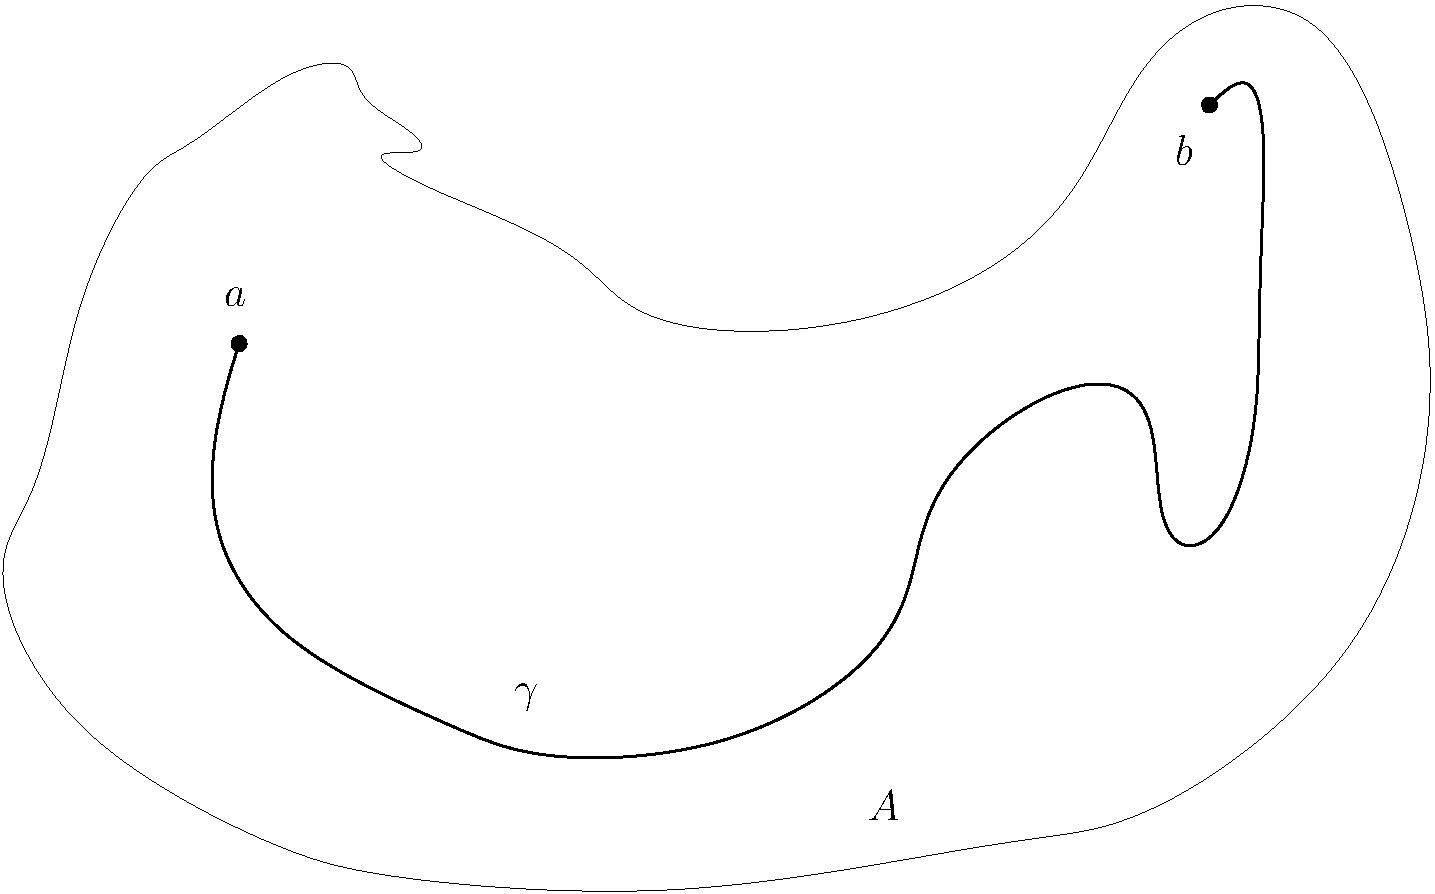
\includegraphics[width=4in]{pathcon.pdf}
\end{center}
The requirement of path-connectedness is stronger than that of connectedness: one can show that every path-connected set is connected, but that the converse is not true.  A common counterexample is the ``topologist's sine curve,'' given as the union of the graph of $\sin(1/x)$ for $x>0$ with the $y$-axis.  However, if we require the set $A$ to be open, then the two notions coincide:
\begin{definition}
A {\bf domain} in $\R^n$ is an open connected subset of $\R^n$.
\end{definition}
\begin{proposition}
A domain is path-connected.
\end{proposition}
While you may not have encountered the notion of connectedness before, it has one very familiar consequence:
\begin{theorem}[The Intermediate Value Theorem]
If a function $f$ is continuous on a set $C$, and $C$ is connected, then $f(C)$ is connected.
\end{theorem}
\begin{proof}
If $f(C)$ were not connected, then there would be sets $U$ and $V$ that define a separation of $f(C)$, and the sets $f^{-1}(U)$ and $f^{-1}(V)$ would be a separation of $C$.
\end{proof}

\section{Homotopy, and simply-connected sets}
\subsection{Deformations of curves}
When discussing problems such as independence of path for line integrals, it is often useful to be able to ``deform'' a given curve $\gamma_1$ into another, simpler curve $\gamma_2$ while leaving the value of the integral along such curves unaffected.  The area of mathematics concerned with such deformations (and higher-dimensional analogues) is called {\em homotopy theory}, and is a branch of algebraic topology.  Typically, we require such deformations to leave the endpoints of the curve unaffected.
\begin{definition}
Let $A\subset \R^n$ be an open connected set. Let $\gamma_0:[0,1]\to A$ and $\gamma_1: [0,1]\to A$ be two continuous curves such that $\gamma_0(0)=\gamma_1(0)=\x_0$ and $\gamma_0(1)=\gamma_1(1)=\x_1$.  We say that $\gamma_0$ and $\gamma_1$ are {\bf homotopic} if there exists a continuous function $H:[0,1]\times [0,1]\to A$, $H(s,t) = \gamma_s(t)$ (called a homotopy between $\gamma_0$ and $\gamma_1$) such that
\begin{enumerate}[(a)]
\item $H(0,t) = \gamma_0(t)$ and $H(1,t) = \gamma_1(t)$,
\item For each $s\in (0,1)$, $H(s,0) = \x_0$ and $H(s,1)=\x_1$,
\item For each $s\in (0,1)$, $H(s,t)$ is a continuous curve contained in $A$.
\end{enumerate}
\end{definition}
In some cases we may require that each of the curves $\gamma_s(t)$ be piecewise-smooth, if $\gamma_0$ and $\gamma_1$ are.  
Homotopies between closed curves are similarly defined, with the exception that instead of requiring the endpoints to remain fixed, we require that $H(s,t)$ be a closed curve for each $s$: $H(s,0)=H(s,1)$ for all $s\in [0,1]$.  
\begin{center}
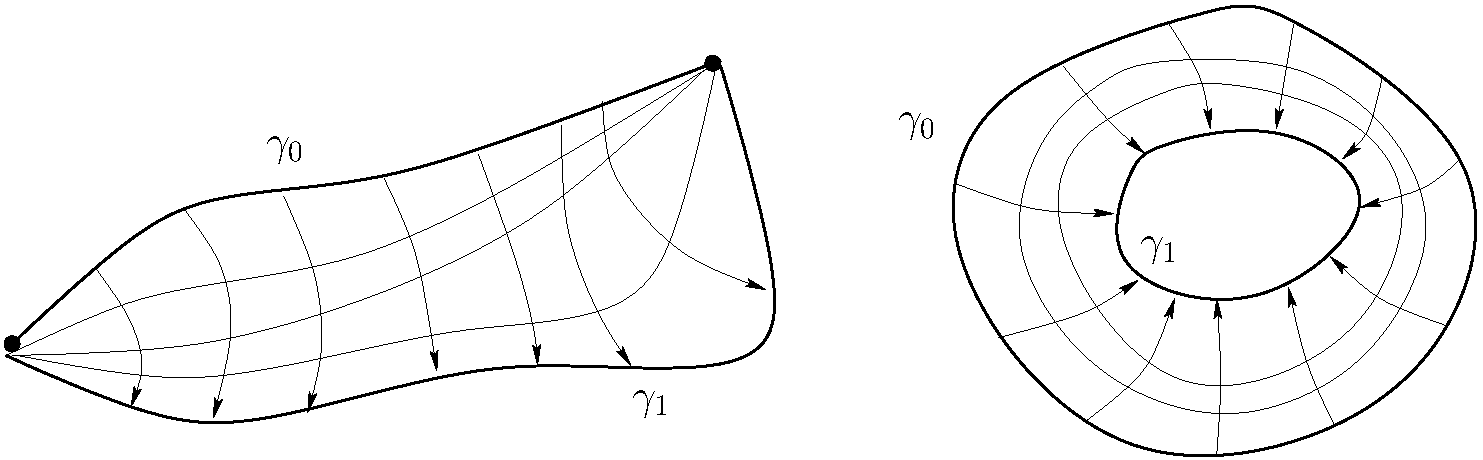
\includegraphics[width=6in]{homotopy.pdf}
\end{center}
If a given simple closed curve $\gamma_0$ can be shrunk to a point (i.e. $\gamma_1(t) = H(1,t) = \x_0$ for all $t$, then we say that $\gamma_0$ is {\em contractible}, or {\em homotopic to a point}.
\begin{definition}
A connected region $A\subseteq \R^n$ is called {\bf simply connected} if any closed curve $\gamma:[0,1]\to A$ is contractible.
\end{definition}
Recall that for $\gamma$ to be contractible, the image of each of the curves $\gamma_s$ has to be contained within $A$.  Thus, in the plane $\R^2$, a simply connected region is intuitively one that has no ``holes'': for example, if $A$ is $\R^2$ minus the origin and $\gamma$ is a closed curve that encircles the origin, then there is no way to shrink $\gamma$ to a point without crossing over the origin, which does not belong to $A$. However, in $\R^3$ (and higher dimensions), simply removing a point does not result in a region that is simply connected, since a curve can now be ``lifted over'' the missing point.

Thus, as we will be able to prove using Stokes' theorem, if a vector field $\mathbf{F}$ in $\R^3$ is defined and $C^1$ except at perhaps finitely many points, then the condition $\nabla\times\mathbf{F}=\mathbf{0}$ is both necessary and sufficient for $\mathbf{F}$ to be the gradient of a function, while in $\R^2$, this is not the case.
\begin{center}
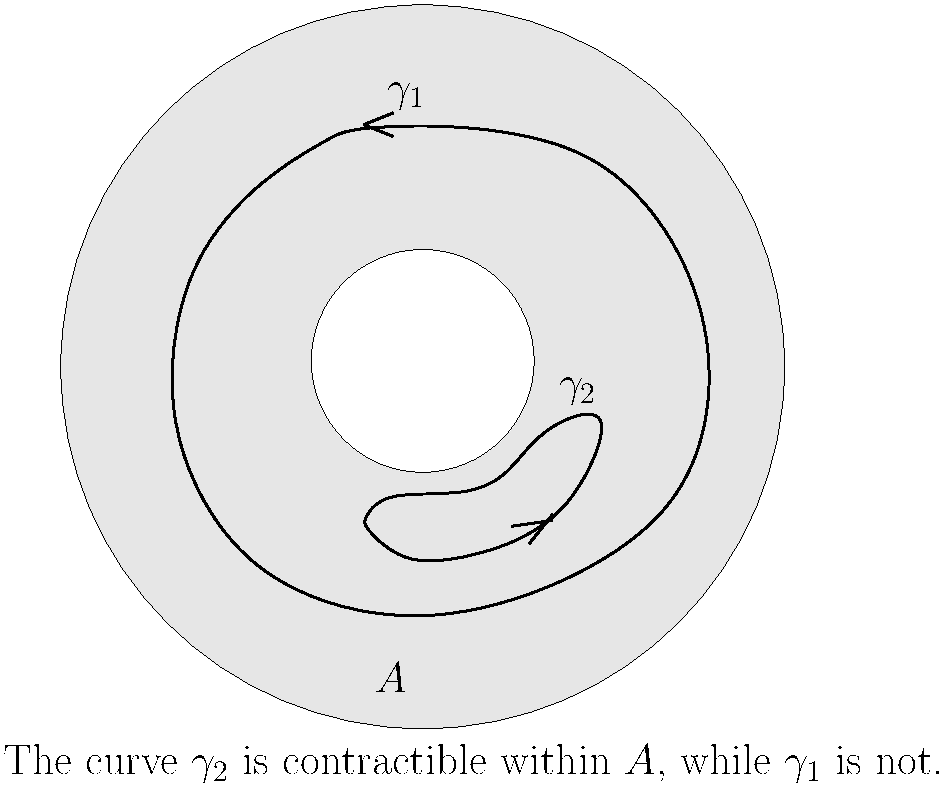
\includegraphics[width=3.5in]{simple.pdf}
\end{center}
A region that is not simply connected is sometimes called {\em multiply connected}.  The origin of this terminology seems to be that we can ``connect'' two points $a$ and $b$ in a path-connected region by some curve; if the region is simply connected then there is only one way to connect $a$ to $b$ ``up to homotopy,'' while in a multiply connected region we can find two non-homotopic paths from $a$ to $b$.  (If $\gamma_1$ and $\gamma_2$ are both paths from $a$ to $b$, then $\gamma_1-\gamma_2$ is a closed curve, and $\gamma_1$ is homotopic to $\gamma_2$ if and only if $\gamma_1-\gamma_2$ is contractible.) 



\end{document}